In this chapter the study designs of both user studies are presented. Both studies have the aim of unraveling insights about the visualization of temporal uncertainty, but their approaches are wildly different. This is due to the varying research questions they try to answer. For this reason the two designs are presented in the following two separate sections. 

\section{Design of the \textit{Evaluation Study}}
\label{ch:evaluationMethod}
Our \textit{Evaluation Study} is building on the work of \citet{gschwandtner2016visual}. \citet{gschwandtner2016visual} compare different visual encodings for temporal uncertainties in order to find out which representations work best for which kinds of tasks. Our goal, on the other hand, is to evaluate for which kinds of tasks it actually makes sense to additionally visualize the information about the temporal uncertainty at all, i.e. in which cases does the user benefit from it and in which cases is the visualized uncertainty more of a distraction and actually not supporting the user in fulfilling his or her tasks. In order to examine those proposed deliberations, we designed our \textit{Evaluation Study} and implemented it using the EvalBench framework. Figure \ref{fig:EvalBench_GUI} shows an example of the user interface of our study implementation inside EvalBench. \par \medskip

\begin{figure}[H]
	\centering
	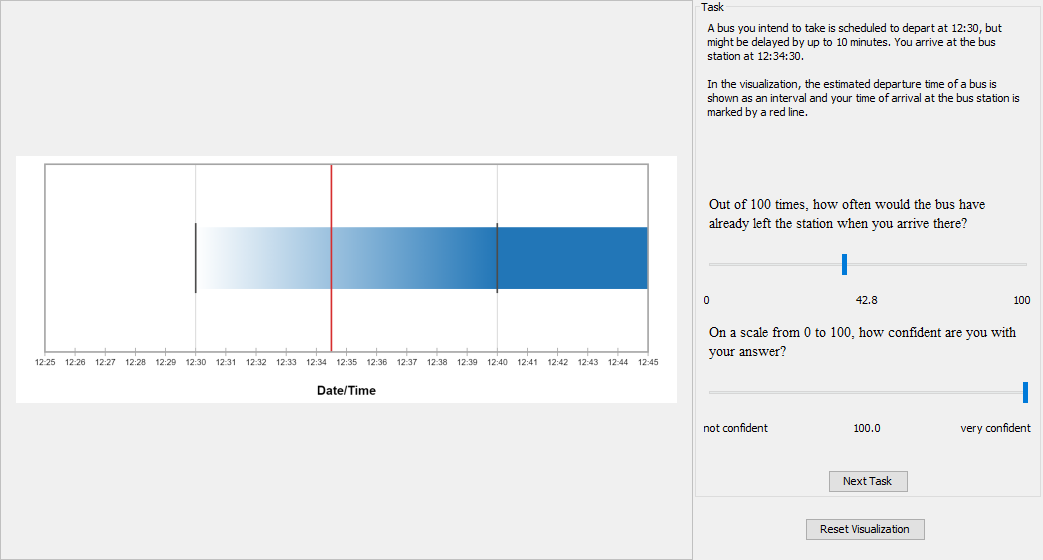
\includegraphics[width=0.95\textwidth]{figures/EvalBench_GUI.png}
	\caption{\textit{A screenshot of our study implementation using EvalBench. On the left side the task supporting visualization is depicted. On the right side the task description and inputs for answers are displayed.}}
	\label{fig:EvalBench_GUI}
\end{figure}

The study was conducted on 3 different user groups. We applied a within-subject-design on the tasks and a between-subject-design on the visualization type. Hence, all participants had to solve the same tasks, but depending on the assigned user group, the participants got different kinds of visualizations, supporting them in fulfilling their tasks. The first user group got Gradient Plots, the second user group got Ambiguation Plots, and the third user group only got visualized mean values, so no visual information about the temporal uncertainty was given at all. However, textual information of the uncertainty intervals, was always provided in the task description for all user groups. \par \medskip

We defined four different task types representing typical questions which might be asked when it comes to temporal uncertainties. Therefore, our study consists of four sequential sessions, covering a wide range of possible tasks. For the first task type, the uncertainty interval of the start- or finish-time of some uncertain time event is given. Furthermore there is a specified point in time, usually lying somewhere inside the uncertainty interval. The participants now have to estimate the probability of the time event having already started or ended at this specified point in time. Figure \ref{fig:EvalBench_session1} shows how tasks of the first session look like for all user groups and how the answer is selected by the participant. Additionally to the task related question, we are also asking for the participant's confidence in his or her given answer. \par \medskip

For the second task type, there are always two parallel uncertainty intervals showing the uncertain finish-times of two possible time events. Again, there is a specified point in time. In these tasks, the participants have to compare the probabilities of both time events at the specified point in time and decide for which uncertainty interval the probability is higher. Figure \ref{fig:EvalBench_session2} shows how tasks of the second session look like and how the answer is selected. \par \medskip

\begin{figure}[H]
	\centering
	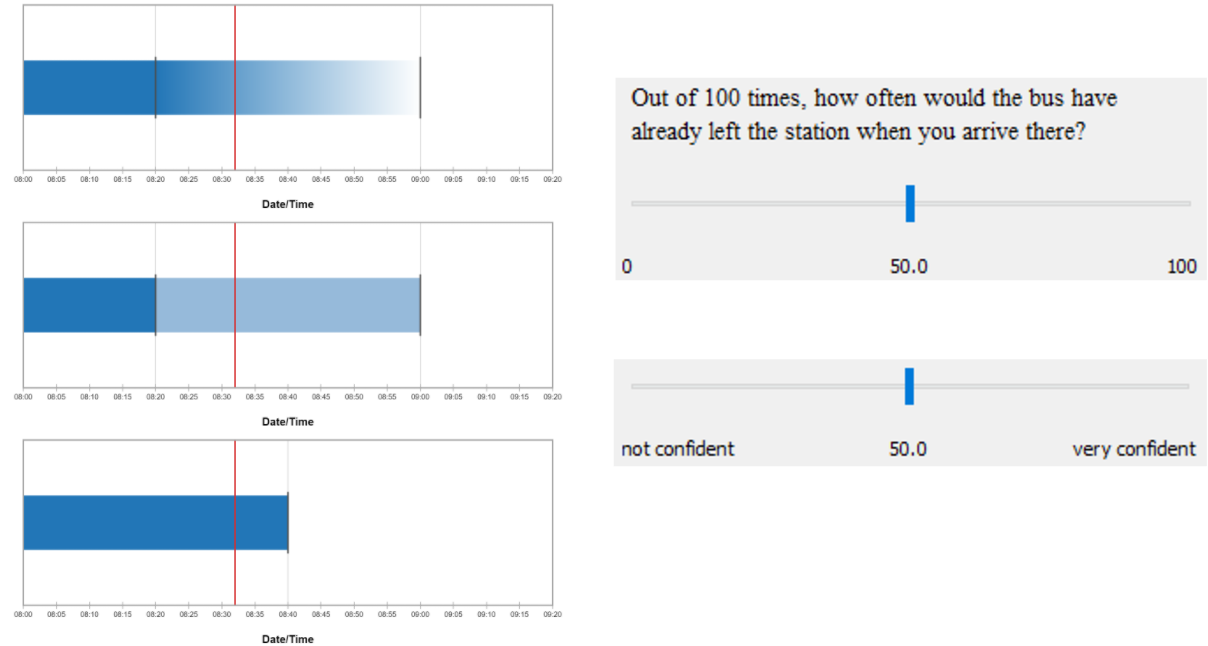
\includegraphics[width=0.9\textwidth]{figures/EvalBench_session1.png}
	\caption{\textit{On the left side the different task supporting visualizations for the first session are shown - from top to bottom: Gradient Plots, Ambiguation Plots, mean values. The specified point in time is marked by a red line in all plots. On the right side, there is an extract of the user interface showing the input fields for giving answers. We are not asking for a percentage value, but for some natural count instead, like suggested by \citet{hullman2016evaluating}.}}
	\label{fig:EvalBench_session1}
\end{figure}

\begin{figure}[H]
	\centering
	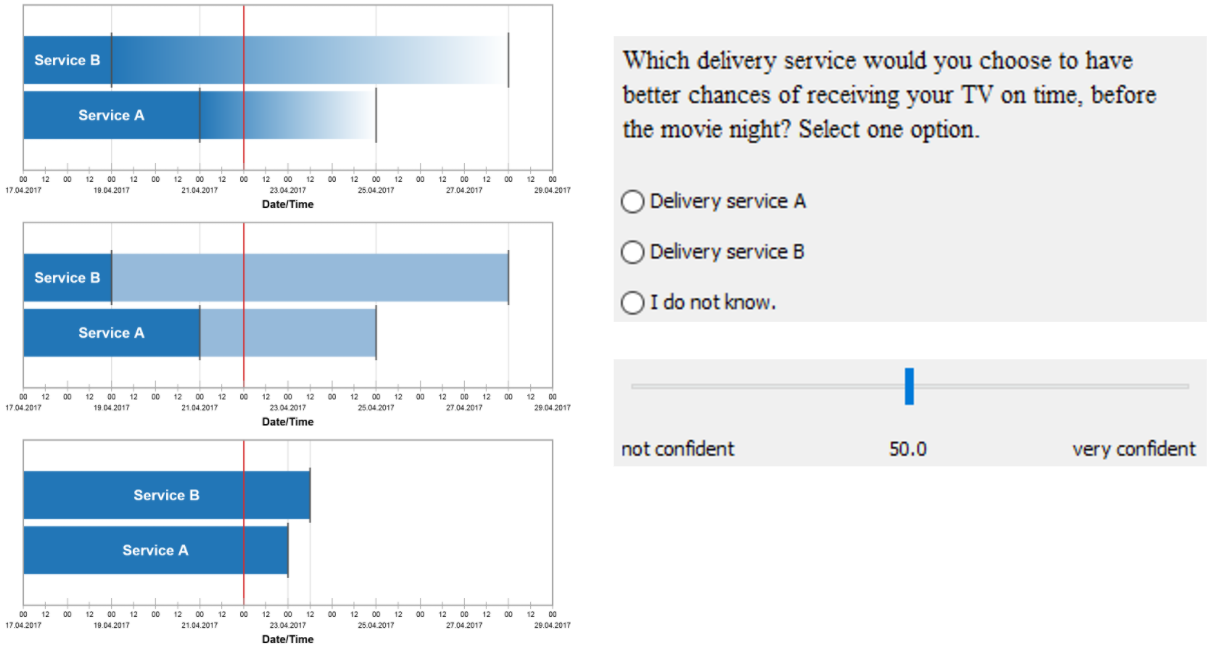
\includegraphics[width=0.9\textwidth]{figures/EvalBench_session2.png}
	\caption{\textit{On the left side the different task supporting visualizations for the second session are shown - from top to bottom: Gradient Plots, Ambiguation Plots, mean values. The specified point in time is marked by a red line in all plots. On the right side, there is an extract of the user interface showing the input fields for giving answers. The answer, i.e. the time event with the estimated higher probability, is selected from a set of radio buttons.}}
	\label{fig:EvalBench_session2}
\end{figure}

For the third session, tasks are similar to the second session. Again, there are two parallel uncertainty intervals showing uncertain finish-times. However, this time there is no specified point in time, but instead the participants are asked to estimate which event will finish sooner on average. Figure \ref{fig:EvalBench_session3} shows how tasks of the third session look like and how the answer is selected. \par \medskip

In the fourth session, tasks revolve around overlapping uncertainty intervals of two successive event. So there is some time event with an uncertain finish-time and some time event with an uncertain start-time and those time events are overlapping to some extent. Here the participants have to estimate the probability of the overlap. Figure \ref{fig:EvalBench_session4} shows how tasks of the fourth session look like and how the answer is selected. \par \medskip

\begin{figure}[H]
	\centering
	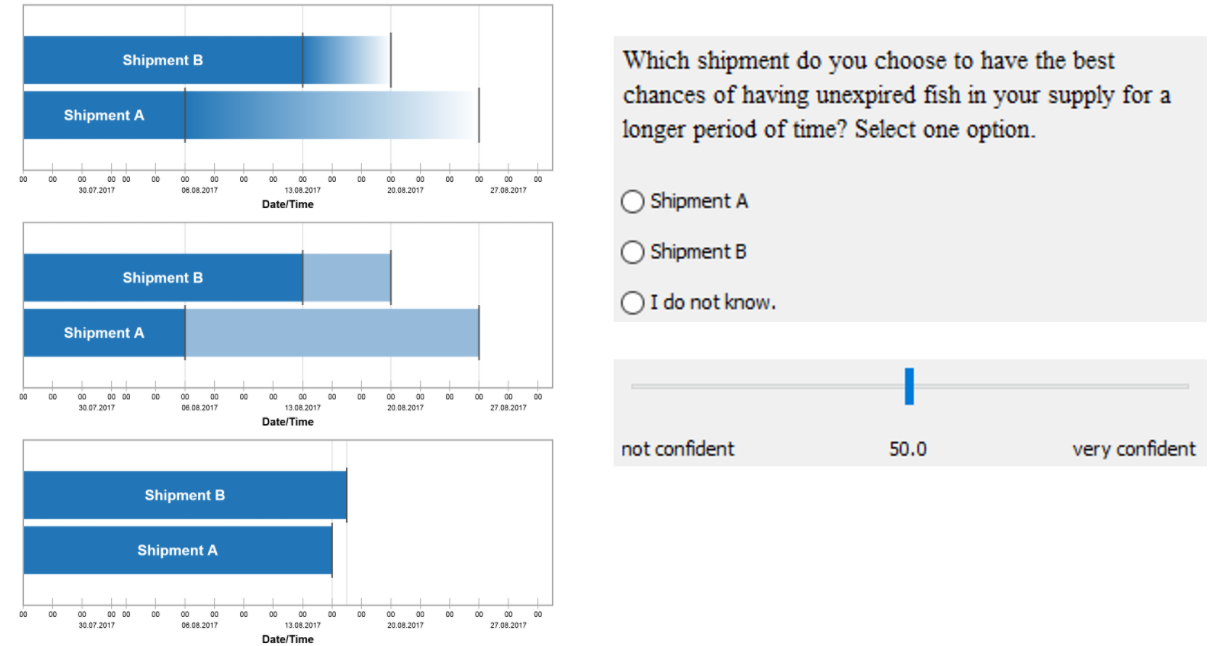
\includegraphics[width=0.9\textwidth]{figures/EvalBench_session3.png}
	\caption{\textit{On the left side the different task supporting visualizations for the third session are shown - from top to bottom: Gradient Plots, Ambiguation Plots, mean values. On the right side, there is an extract of the user interface showing the input fields for giving answers. The answer, i.e. the time event which is estimated to end sooner, is selected from a set of radio buttons.}}
	\label{fig:EvalBench_session3}
\end{figure}

\begin{figure}[H]
	\centering
	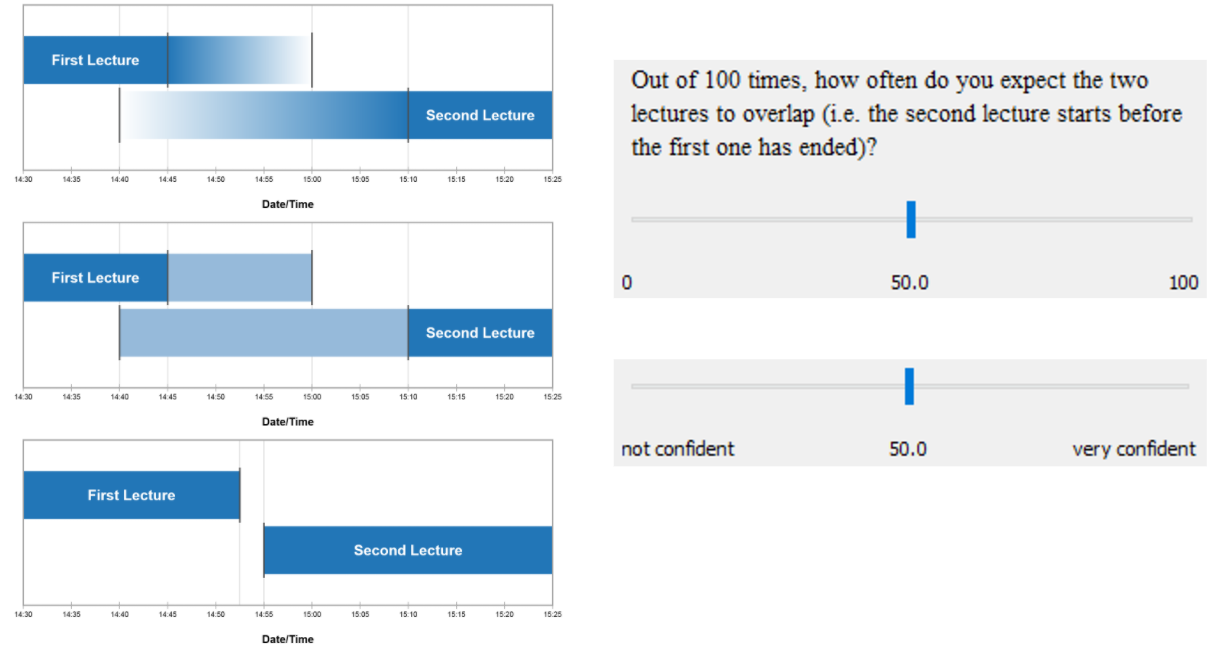
\includegraphics[width=0.9\textwidth]{figures/EvalBench_session4.png}
	\caption{\textit{On the left side the different task supporting visualizations for the fourth session are shown - from top to bottom: Gradient Plots, Ambiguation Plots, mean values. On the right side, there is an extract of the user interface showing the input fields for giving answers. Like in the first session, we are again not asking for a percentage value, but for some natural count instead, like suggested by \citet{hullman2016evaluating}.}}
	\label{fig:EvalBench_session4}
\end{figure}

TODO - Hypothesen hier oder in results?


\section{Design of the \textit{Drawing Study}}
\label{ch:drawingMethod}
The \textit{Drawing Study} is designed to be of exploratory nature. This means that the research question it aims to answer is not as concrete as for instance the one of our \textit{Evaluation Study}. The goal is to gain insights into the intuitiveness of visual encodings and to find out how people would visualize temporal uncertainty by themselves. This information could consequently be used in the design of novel visualizations, aimed at expert and especially non-expert users. \par \medskip

To gain these insights, we describe predefined scenarios, which encompass some kind of temporal uncertainty, to our study participants and ask them to draw a visualization sketch that intuitively represents this given scenario. Furthermore, the participants are always provided with a certain task a hypothetical user should be able to efficiently solve given an implementation of the sketched design. \par \medskip

To elicit the desired sketches of temporal visualizations from our study participants, we have to ask the right questions and also have to pay close attention to ask them in the right way. This means that it is imperative to not suggest any possible answers or solution approaches while communicating the task that should be solved, because this would greatly affect their given answers \cite{hullman2016evaluating}. For this reason we try our best to make the given scenario and the task as clear as possible to our participant without suggesting anything that would help in the solution of the task. \par \medskip

\section{Participants}
\label{ch:participants}
In sum we had 32 participants. Two of them only participated in the \textit{Drawing Study}, but not in the \textit{Evaluation Study}. Hence, we collected 30 and 32 datasets for the two studies respectively. \par \medskip

The participants were chosen people from our friends and family. To make the results as representative as possible, we tried to recruit a heterogeneous group. 20 of our participants are male, while 12 of them are female. Recruiting a heterogeneous group in terms of age was not as easy. We ended up with 24 people under the age of 30 and 8 older ones. \par \medskip

To further given an idea of the participant's demographic we estimated their daily computer usage and knowledge in the field of information visualization and ranked those two factors from in the categories low, average and high. Our participant group shows a rather high density of heavy computer users, with a sum of 17 of them. 10 of them are ranked as average users and only 5 of them use computers seldom. \par \medskip

Since some of the recruited participant are study colleagues of us and also study computer science, they have some knowledge about information visualization. In sum 5 of them completed a bachelor course about this topic and were therefore ranked 'high' by us. 11 participants were ranked average, because they either encounter many data visualizations in their daily work life or studied something technical that involves such visualizations, even though there is no specific information visualization course. The remaining 16 users have no education in this field and work with visualizations only seldom. \par \medskip

An overview of the demographic of the participants is presented in Table \ref{tb:participants}.


\begin{table}[]
	\centering
	\resizebox{\textwidth}{!}{%
	\begin{tabular}{lrll|l|r|r|}
		\cline{2-2} \cline{4-4} \cline{6-7}
		\multicolumn{1}{l|}{\textit{\textbf{Demographic}}} & \multicolumn{1}{r|}{\textbf{Sex}} & \multicolumn{1}{l|}{}             & \textbf{Age}            &                  & \textbf{Computer Usage} & \textbf{InfoVis Knowledge} \\ \hline
		\multicolumn{1}{|l|}{\textit{Male}}                & \multicolumn{1}{r|}{20}           & \multicolumn{1}{l|}{\textit{<30}} & \multicolumn{1}{r|}{24} & \textit{Low}     & 5                       & 16                         \\ \hline
		\multicolumn{1}{|l|}{\textit{Female}}              & \multicolumn{1}{r|}{12}           & \multicolumn{1}{l|}{\textit{>30}} & \multicolumn{1}{r|}{8}  & \textit{Average} & 10                      & 11                         \\ \hline
		& \multicolumn{1}{l}{}              &                                   &                         & \textit{High}    & 17                      & 5                          \\ \cline{5-7} 
	\end{tabular}
}
	\caption{\textit{This table summarizes the demographic of our study participants. A more specific description of it can be found in the \hyperref[ch:participants]{previous section}.}}
	\label{tb:participants}
\end{table}


